%
\documentclass[aspectratio=169]{beamer}

\usepackage{tikz}

\setbeamercovered{invisible}
\usenavigationsymbolstemplate{}


\begin{document}

\begin{frame}

\vspace{-20pt}
\[
\hspace{-2cm}

\begin{tikzpicture}[xscale=1.2, yscale=1.8]
\foreach \x/\y in {0/red,1/orange,2/yellow,3/green,4/blue} {
  \path [fill=\y] (0,\x) rectangle +(\textwidth,1);
}
\path [use as bounding box] (current bounding box.south west) rectangle (current bounding box.north east);
\node [scale=2.5, white, yscale=4.04] at (0.5*\textwidth,2.23) {\Huge\bf QUBIT.ZONE};
\end{tikzpicture}
\hspace{-2cm}
\]

\end{frame}

\usebackgroundtemplate{$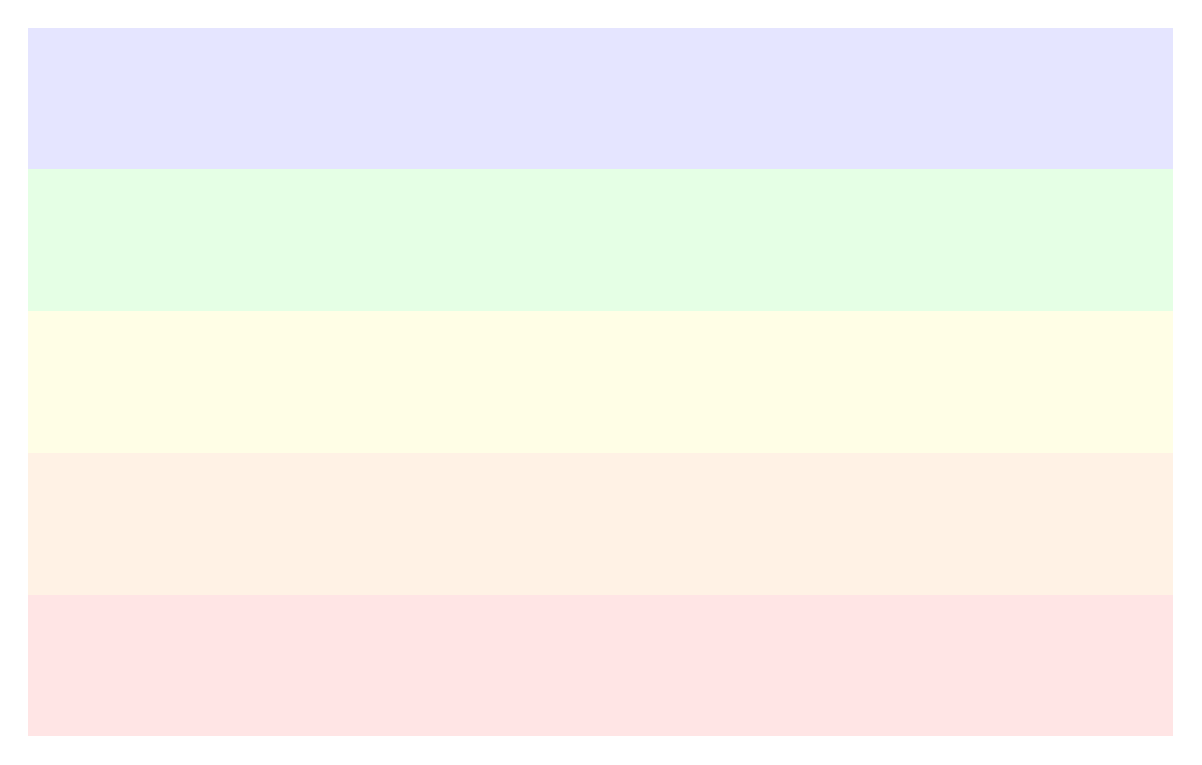
\begin{tikzpicture}[xscale=1.2, yscale=1.8]
\foreach \x/\y in {0/red,1/orange,2/yellow,3/green,4/blue} {
  \path [fill=\y!10] (0,\x) rectangle +(\textwidth,1);
}
\end{tikzpicture}$}


\setbeamertemplate{frametitle}{\color{black}\centering\Huge\bfseries\insertframetitle\par\vskip-6pt}

\begin{frame}
\frametitle{QUANTUM COMPUTERS}

Scientists around the world are racing to build the first \textit{quantum computer}. PICTURE.

\vspace{15pt}
Over the next 100 years, they will transform our civilization, giving us incredible new powers of ... DRUG DESIGN, OPTIMIZATION, DATA ANALYSIS, BREAKING ENCRYPTION, ARTIFICIAL INTELLIGENCE. [INSERT PICTURES FROM DALHOUSIE TALK.]

\end{frame}

\begin{frame}
\frametitle{QUBITS}

Ordinary computers are built from \textit{bits}, which can equal 0 or 1. PICTURE.

\vspace{10pt}
Quantum computers will be built from \textit{qubits}. You've got one in front of you!
\[
\text{[PICTURE]}
\]
It has got lots of mysterious buttons. Give them a try.

\vspace{10pt}
We will use these later to \textit{program} the qubit.

\end{frame}

\begin{frame}
\frametitle{plan}

\begin{itemize}
\item Superposition
\item Entanglement
\item Dense coding
\item Entanglement
\item Teleportation
\end{itemize}



\end{frame}

\end{document}\end{document}\end{document}

\begin{frame}
\section{Qubits}

\paragraph{What is a qubit?}

Scientists around the world are racing to build the first quantum computer, which will use the laws of quantum mechanics to solve some problems much faster than any computer we have now. Using your very own qubit, we can investigate some of the 

While today's computers store information using bits, quantum computers will store information using qubits

...

 - A qubit is the basic building block of a quantum computer
 
 - Measure, one-qubit operations, two-qubit operations
 
 - Using the cable
 
 - All the operations cancel themselves out if you do them twice. So if you press one by accident, press it again
 
 \section{Measurement}
 
You can ask a qubit the following question: ``what state are you in?''. The answer will be 0 or 1.

\section{Superposition}



\section{Entanglement}

Two entangled qubits will behave the same way, however far separated they are in space.

\paragraph{Experiment.} Entangle two qubits, then measure each of them.

\section{Teleportation}

\paragraph{Experiment.} 

\section{Super Dense Coding}

We can use qubits to send messages, by 

\end{frame}

\end{document}
